% !TEX root =  paper.tex
\section{Background}\label{sec:background}

\lstset{
	emphstyle=\color{blue}\bfseries,
	numbers=left,
	%basicstyle=\ttfamily,
	basicstyle=\linespread{0.7}\fontsize{6}{12}\selectfont\ttfamily,
	numberstyle=\scriptsize,
	stepnumber=1,
	language=Java,
	numbersep=8pt,
	keywordstyle=\color{blue}\bfseries,
	commentstyle=\color{mygreen},
	stringstyle=\color{orange2},
	%frameround=fttt,
	%frame=trBL,
	frame=lines,
	captionpos=b,
	backgroundcolor=\color{lightgray},
	tabsize=3,
}

\begin{figure}[tb]
\centering
\begin{subfigure}{\linewidth}
\centering
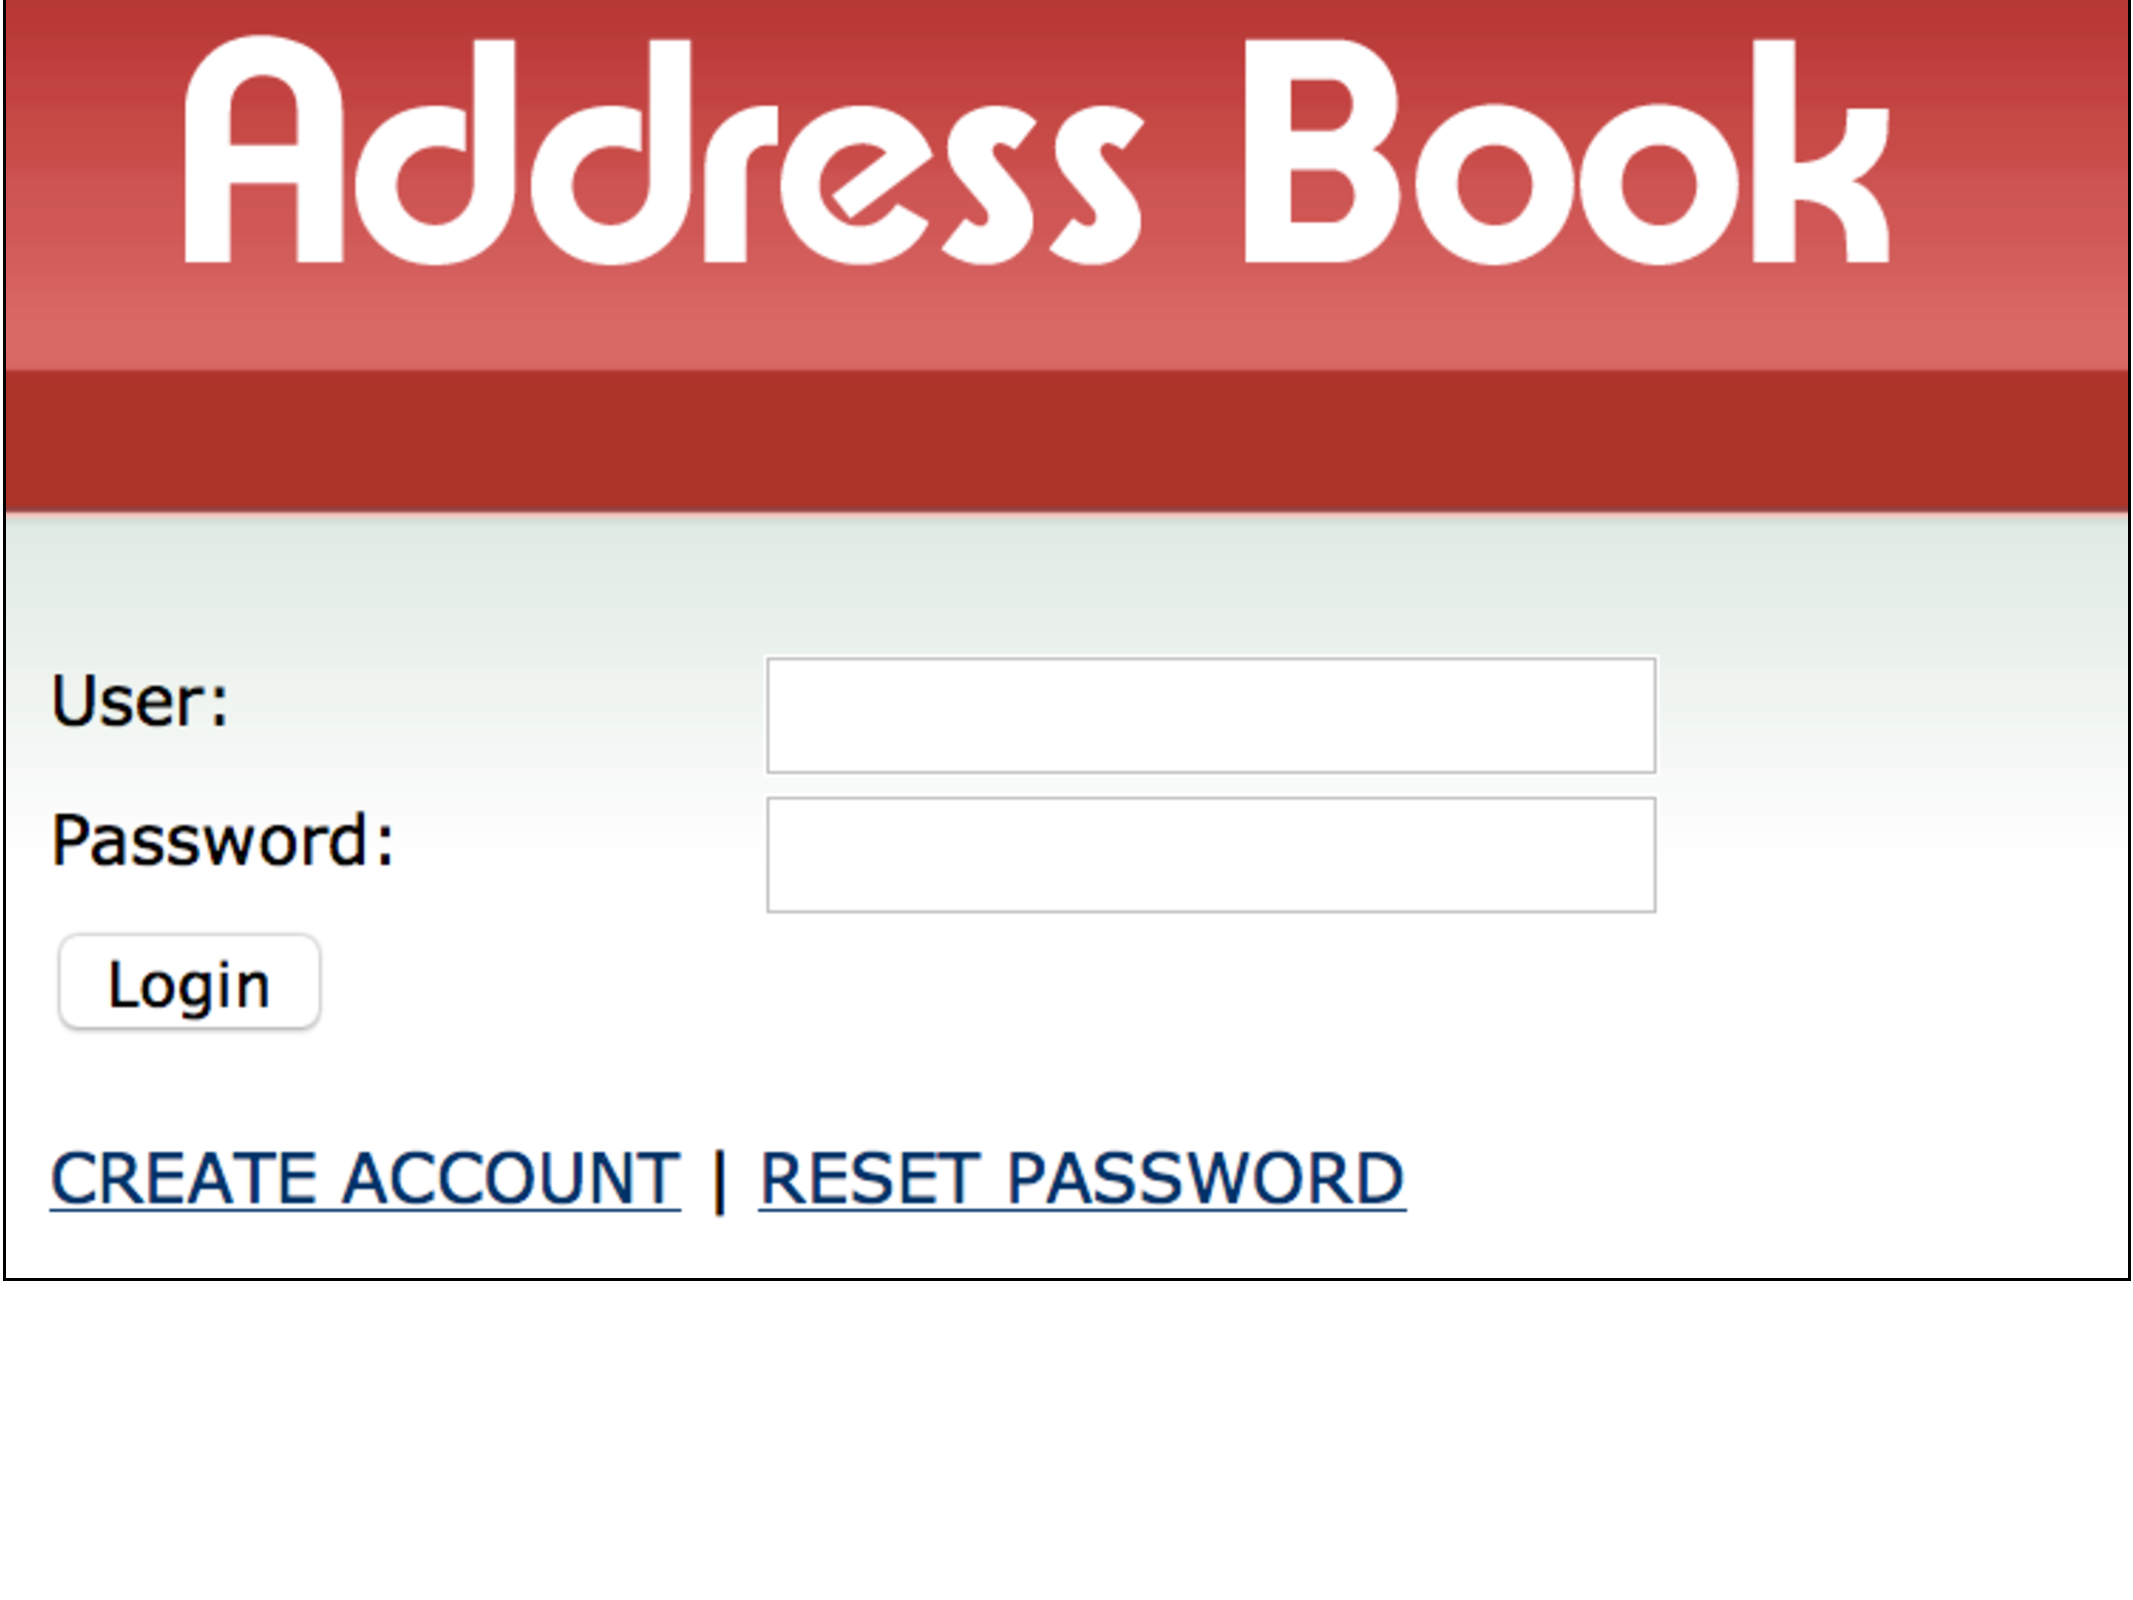
\includegraphics[trim=0.1cm 5cm 0.1cm 0.1cm, clip=true, scale=0.16]{images/ab1.pdf}
\caption{\emph{Login page.}}
\label{fig:ab-back-a} 
\end{subfigure}
\begin{subfigure}{\linewidth}
\centering
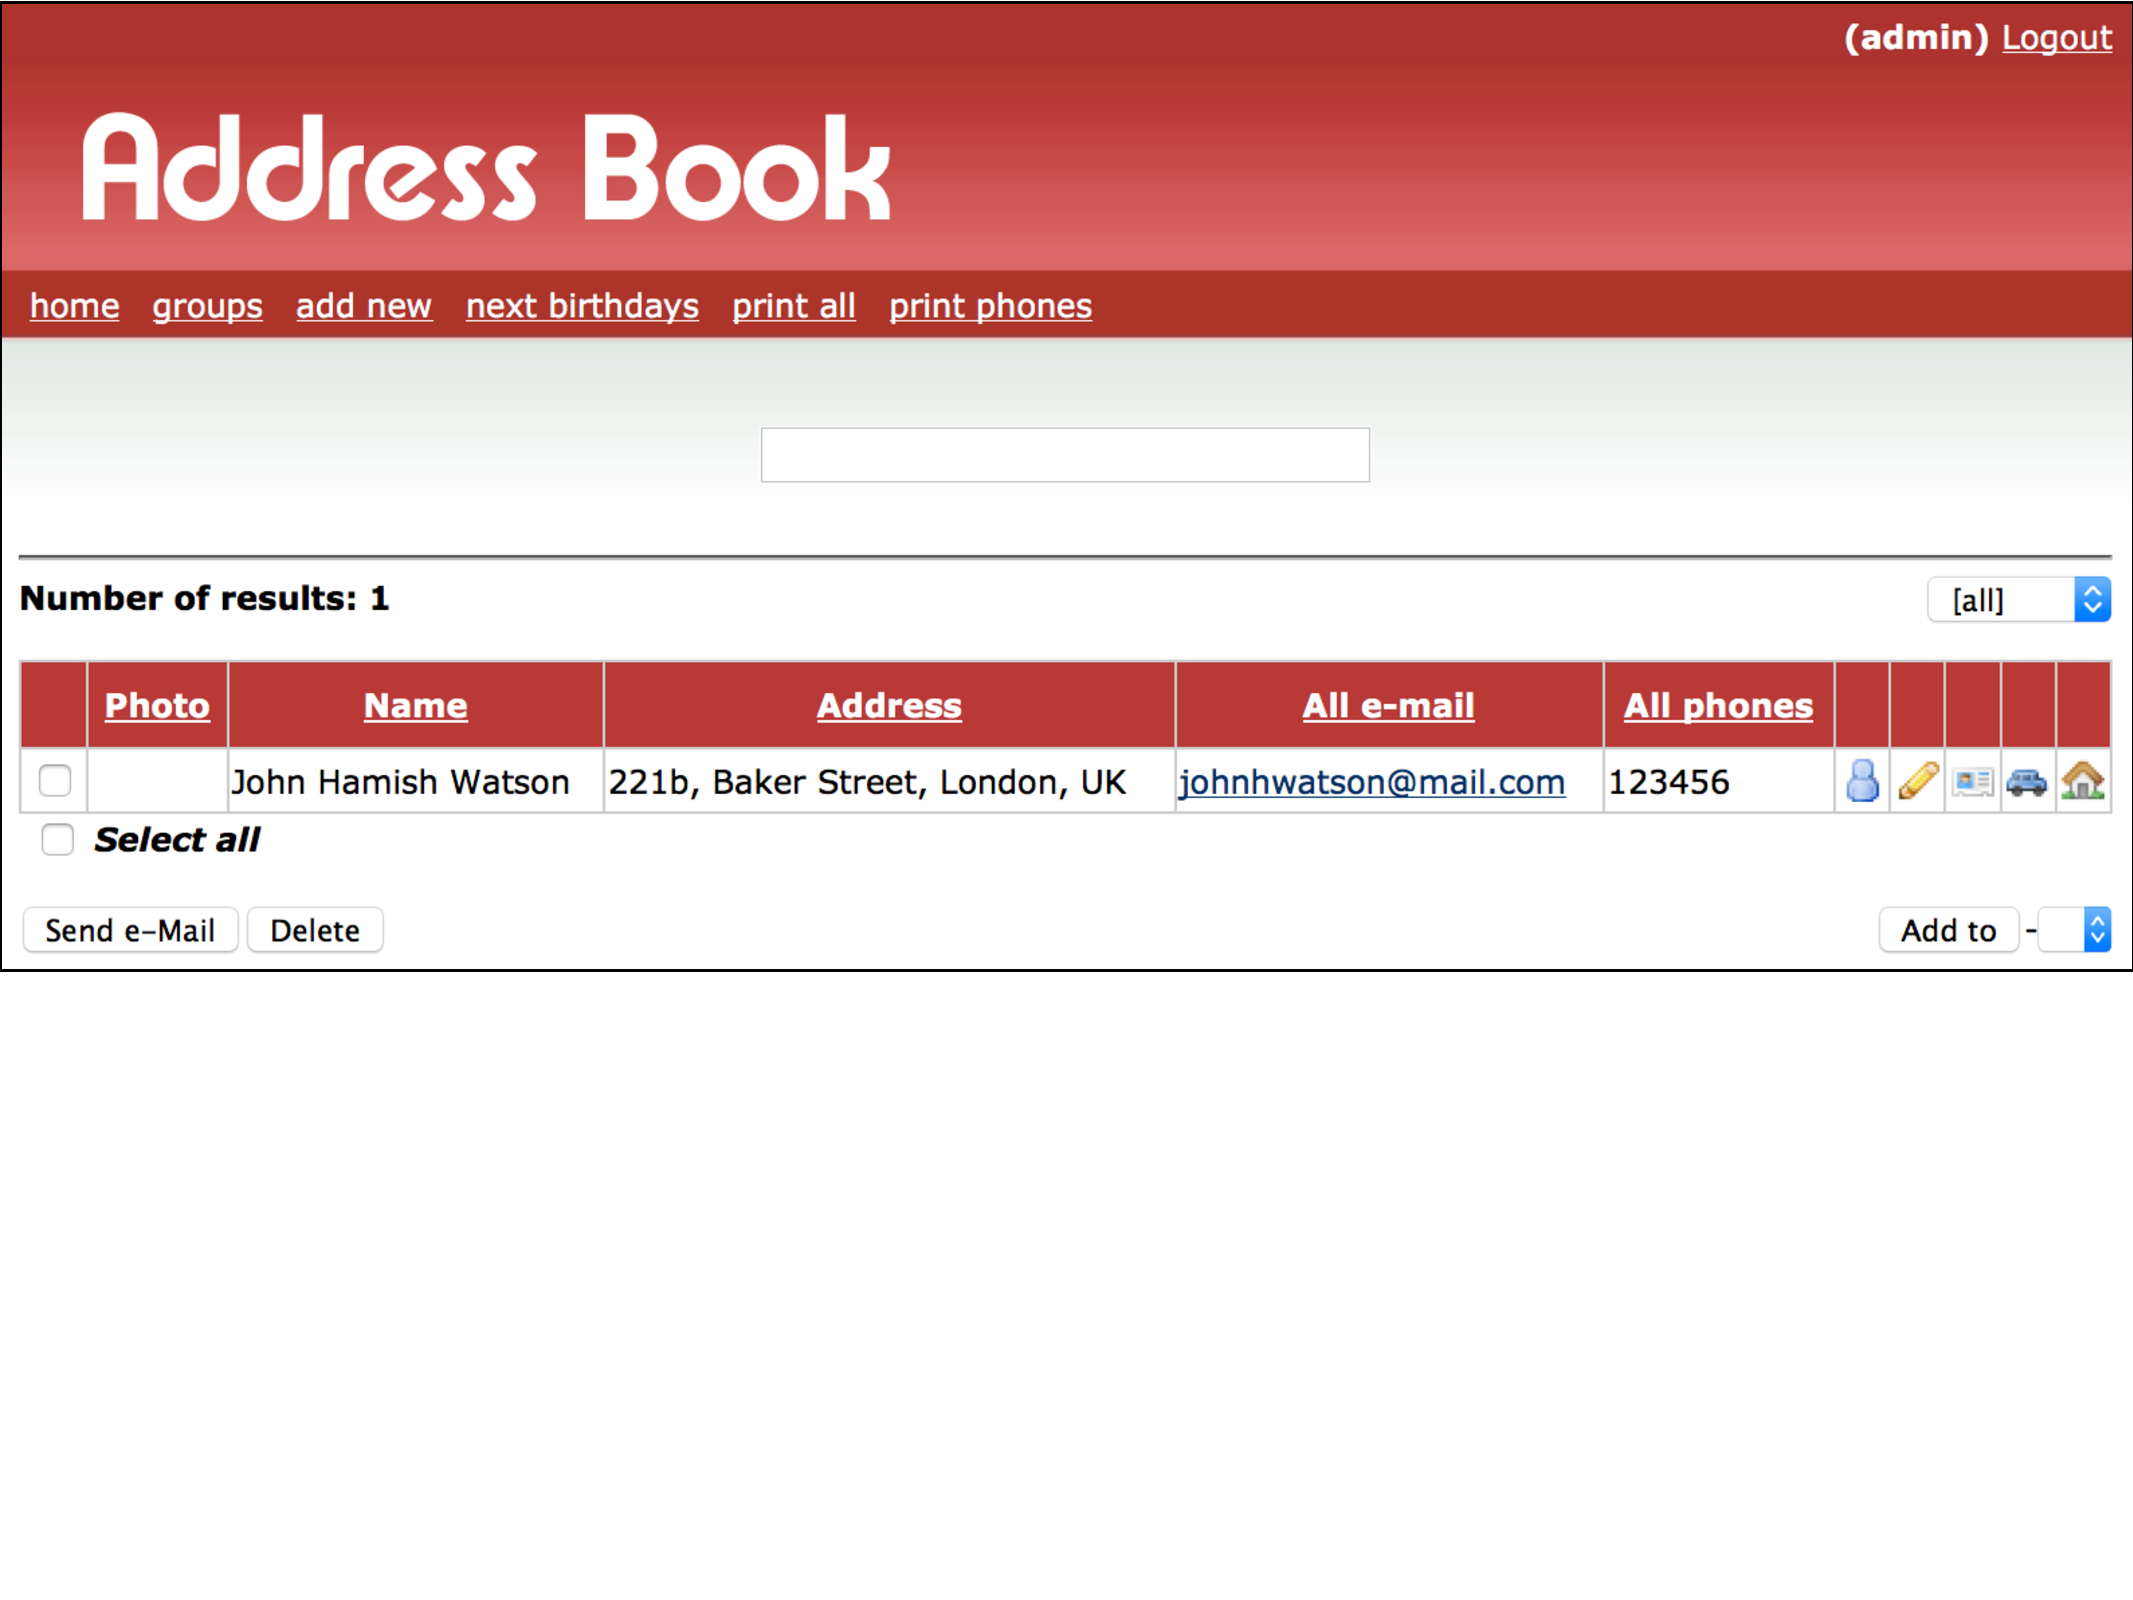
\includegraphics[trim=0cm 10.5cm 0cm 0cm, clip=true, scale=0.22]{images/ab2.pdf}  \caption{\emph{Home page.}}
\label{fig:ab-back-b} 
\end{subfigure}
\caption{AddressBook web application}
\label{fig:ab-back}
\end{figure}

%\begin{table*}%[h]
\setlength{\tabcolsep}{3pt}
\renewcommand{\arraystretch}{0.9}
\centering
\caption{Web Breakages and Root Causes}
\begin{threeparttable}
\begin{tabular}{l@\qquad l@\qquad ccc}
\toprule
\bf Distal Cause & \bf Proximal Cause  & \multicolumn{3}{c}{\bf Impact} \\
\cmidrule(r){3-5}
 &  &  \bf DOM & \bf GUI & \bf workflow \\
\textsc{Addition} &  &   &  &  \\
\quad A web element $e$ has been inserted & test value/action & y & y & y \\
\quad A popup window $p$ has been inserted & popup &  n & y & y \\[0.5ex]
\textsc{Deletion} &  &  &  &  \\
\quad An attribute $a$ of a web element $e$* has been deleted & attribute locator &  y & y/n & y/n \\
\quad A textual content $t$ of a web element $e$ has been deleted & assertion value &  y & y & y \\
\quad A value/statement $v$ has become obsolete & test value/action &  y & y & y \\
\quad A web element $e$ has been deleted & locator and value/action &  y & y & y \\[0.5ex]
\textsc{Modification} &  &  &  &  \\
\quad An attribute $a$ of a web element $e$ has been modified & attribute locator &  y & n & y/n \\
\quad A textual content $t$ of a web element $e$** has been modified & assertion value &  y & y & n \\
\quad The web app structure or a tag of a web element $e$ have been changed & hierarchy based locator &  y & y/n & y/n \\
\quad A web element $e$ is repositioned on the page & position based locator &  y & y & y/n \\
\quad A value $v$ has become obsolete, or assertion invalid & test value/action &  y & y & y/n \\
\bottomrule
\end{tabular}
\begin{tablenotes}
    \item\text{*} = value absent from ddl
    \item\text{**} = unexpected assertion value
\end{tablenotes}
\end{threeparttable}
\label{table:rootcauses}
\end{table*}

%\begin{table*}%[h]
%\setlength{\tabcolsep}{3pt}
%\renewcommand{\arraystretch}{0.9}
%\centering
%\caption{Web Breakages and Root Causes}
%\begin{threeparttable}
%\begin{tabular}{lllccc}
%\toprule
%\bf Proximal Cause & \bf Related to & \bf Distal Cause & \multicolumn{3}{c}{\bf Impact} \\
%\cmidrule(r){4-6}
% &  &  & \bf DOM & \bf GUI & \bf workflow \\
%\textsc{Addition} &  &  &  &  &  \\
%\quad test value/action & value/statement & A value/statement has become necessary & y & y & y \\
%\quad popup & popup window & A popup window has been inserted & n & y & y \\[0.5ex]
%\textsc{Deletion} &  &  &  &  &  \\
%\quad attribute & attribute of a web element $e$* & Attribute $a$ has been deleted & y & y/n & y/n \\
%\quad text & textual content of a web element $e$ & Text content $t$ has been deleted (rare) & y & y & y \\
%\quad hierarchy & web element $e$ & web app structure has been changed or tag changed & y & y/n & y/n \\
%\quad index position & web element $e$ & an element is repositioned on the page & y & y & y/n \\
%\quad value/action & value/statement & A value/statement has become obsolete & y & y & y \\
%\quad web element & web element $e$ & web element has been deleted & y & y & y \\[0.5ex]
%\textsc{Modification} &  &  &  &  &  \\
%\quad attribute & attribute of a web element $e$ & Attribute $a$ has been modified & y & n &  \\
%\quad text & textual content of a web element $e$** & Text content $t$ has been modified & y & y & n \\
%\quad test value/action & value/statement & A value has become obsolete, or assertion invalid & ? & ? & y \\
%%*value absent from ddl &  &  &  &  &  \\
%%**unexpected assertion value &  &  &  &  & \\
%\bottomrule
%\end{tabular}
%\begin{tablenotes}
%    \item\text{*} = value absent from ddl
%    \item\text{**} = unexpected assertion value
%\end{tablenotes}
%\end{threeparttable}
%\label{table:rootcauses}
%\end{table*}
%\begin{table*}%[h]
\setlength{\tabcolsep}{3pt}
\renewcommand{\arraystretch}{0.9}
\centering
\caption{Examples of Root Causes}
\begin{tabular}{l@\qquad l}
\toprule
\bf Distal Cause & \bf Example \\
\textsc{Addition} &  \\
\quad A web element $e$ has been inserted & AddressBook v.6.2.11 $\rightarrow$ v8.2.5 Next button \\
\quad A popup window $p$ has been inserted & PHPFusion v.7.0.0 assertion message $\rightarrow$ popup message \\[0.5ex]
\textsc{Deletion} &  \\
\quad An attribute $a$ of a web element $e$* has been deleted & attribute locator \\
\quad A textual content $t$ of a web element $e$ has been deleted (rare) & assertion cannot be repaired! \\
\quad A value/statement $v$ has become obsolete & test value/action \\
\quad A web element $e$ has been deleted & locator and value/action \\[0.5ex]
\textsc{Modification} &  \\
\quad An attribute $a$ of a web element $e$ has been modified & attribute locator  \\
\quad A textual content $t$ of a web element $e$** has been modified & assertion value \\
\quad The web app structure or a tag of a web element $e$ have been changed & hierarchy based locator  \\
\quad A web element $e$ is repositioned on the page & position based locator \\
\quad A value $v$ has become obsolete, or assertion invalid & test value/action \\
\bottomrule
\end{tabular}
\label{table:examples}
\end{table*}
%\begin{table*}%[h]
\setlength{\tabcolsep}{3pt}
\renewcommand{\arraystretch}{0.9}
\centering
\caption{Examples of Root Causes}
\begin{tabular}{l@\qquad l}
\toprule
\bf Distal Cause & \bf Example \\
\textsc{Addition} &  \\
\quad A web element $e$ has been inserted & AddressBook v.6.2.11 $\rightarrow$ v8.2.5 Next button \\
\quad A popup window $p$ has been inserted & PHPFusion v.7.0.0 assertion message $\rightarrow$ popup message \\[0.5ex]
\textsc{Deletion} &  \\
\quad An attribute $a$ of a web element $e$* has been deleted & attribute locator \\
\quad A textual content $t$ of a web element $e$ has been deleted (rare) & assertion cannot be repaired! \\
\quad A value/statement $v$ has become obsolete & test value/action \\
\quad A web element $e$ has been deleted & locator and value/action \\[0.5ex]
\textsc{Modification} &  \\
\quad An attribute $a$ of a web element $e$ has been modified & attribute locator  \\
\quad A textual content $t$ of a web element $e$** has been modified & assertion value \\
\quad The web app structure or a tag of a web element $e$ have been changed & hierarchy based locator  \\
\quad A web element $e$ is repositioned on the page & position based locator \\
\quad A value $v$ has become obsolete, or assertion invalid & test value/action \\
\bottomrule
\end{tabular}
\label{table:examples}
\end{table*}

%\begin{lstlisting}[firstnumber=1, xleftmargin=6ex, float=b,numbers=left,caption={Automated test case},label=lst:example]
%@Test
%public void testClarolineLogin(){
%	WebDriver driver = new FirefoxDriver();
%	driver.get("localhost:8080/claroline/");
%	driver.findElement(By.name("user")).sendKeys("admin");
%	driver.findElement(By.name("pass")).sendKeys("admin");
%	driver.findElement(By.name("submitAuth")).click();
%	AssertThat(driver.findElement(By.id("loggedUser")).getText(), is("admin"));
%	driver.quit();
%}
%\end{lstlisting}
%
%\begin{figure}[t]
%\centering
%%\fbox{
%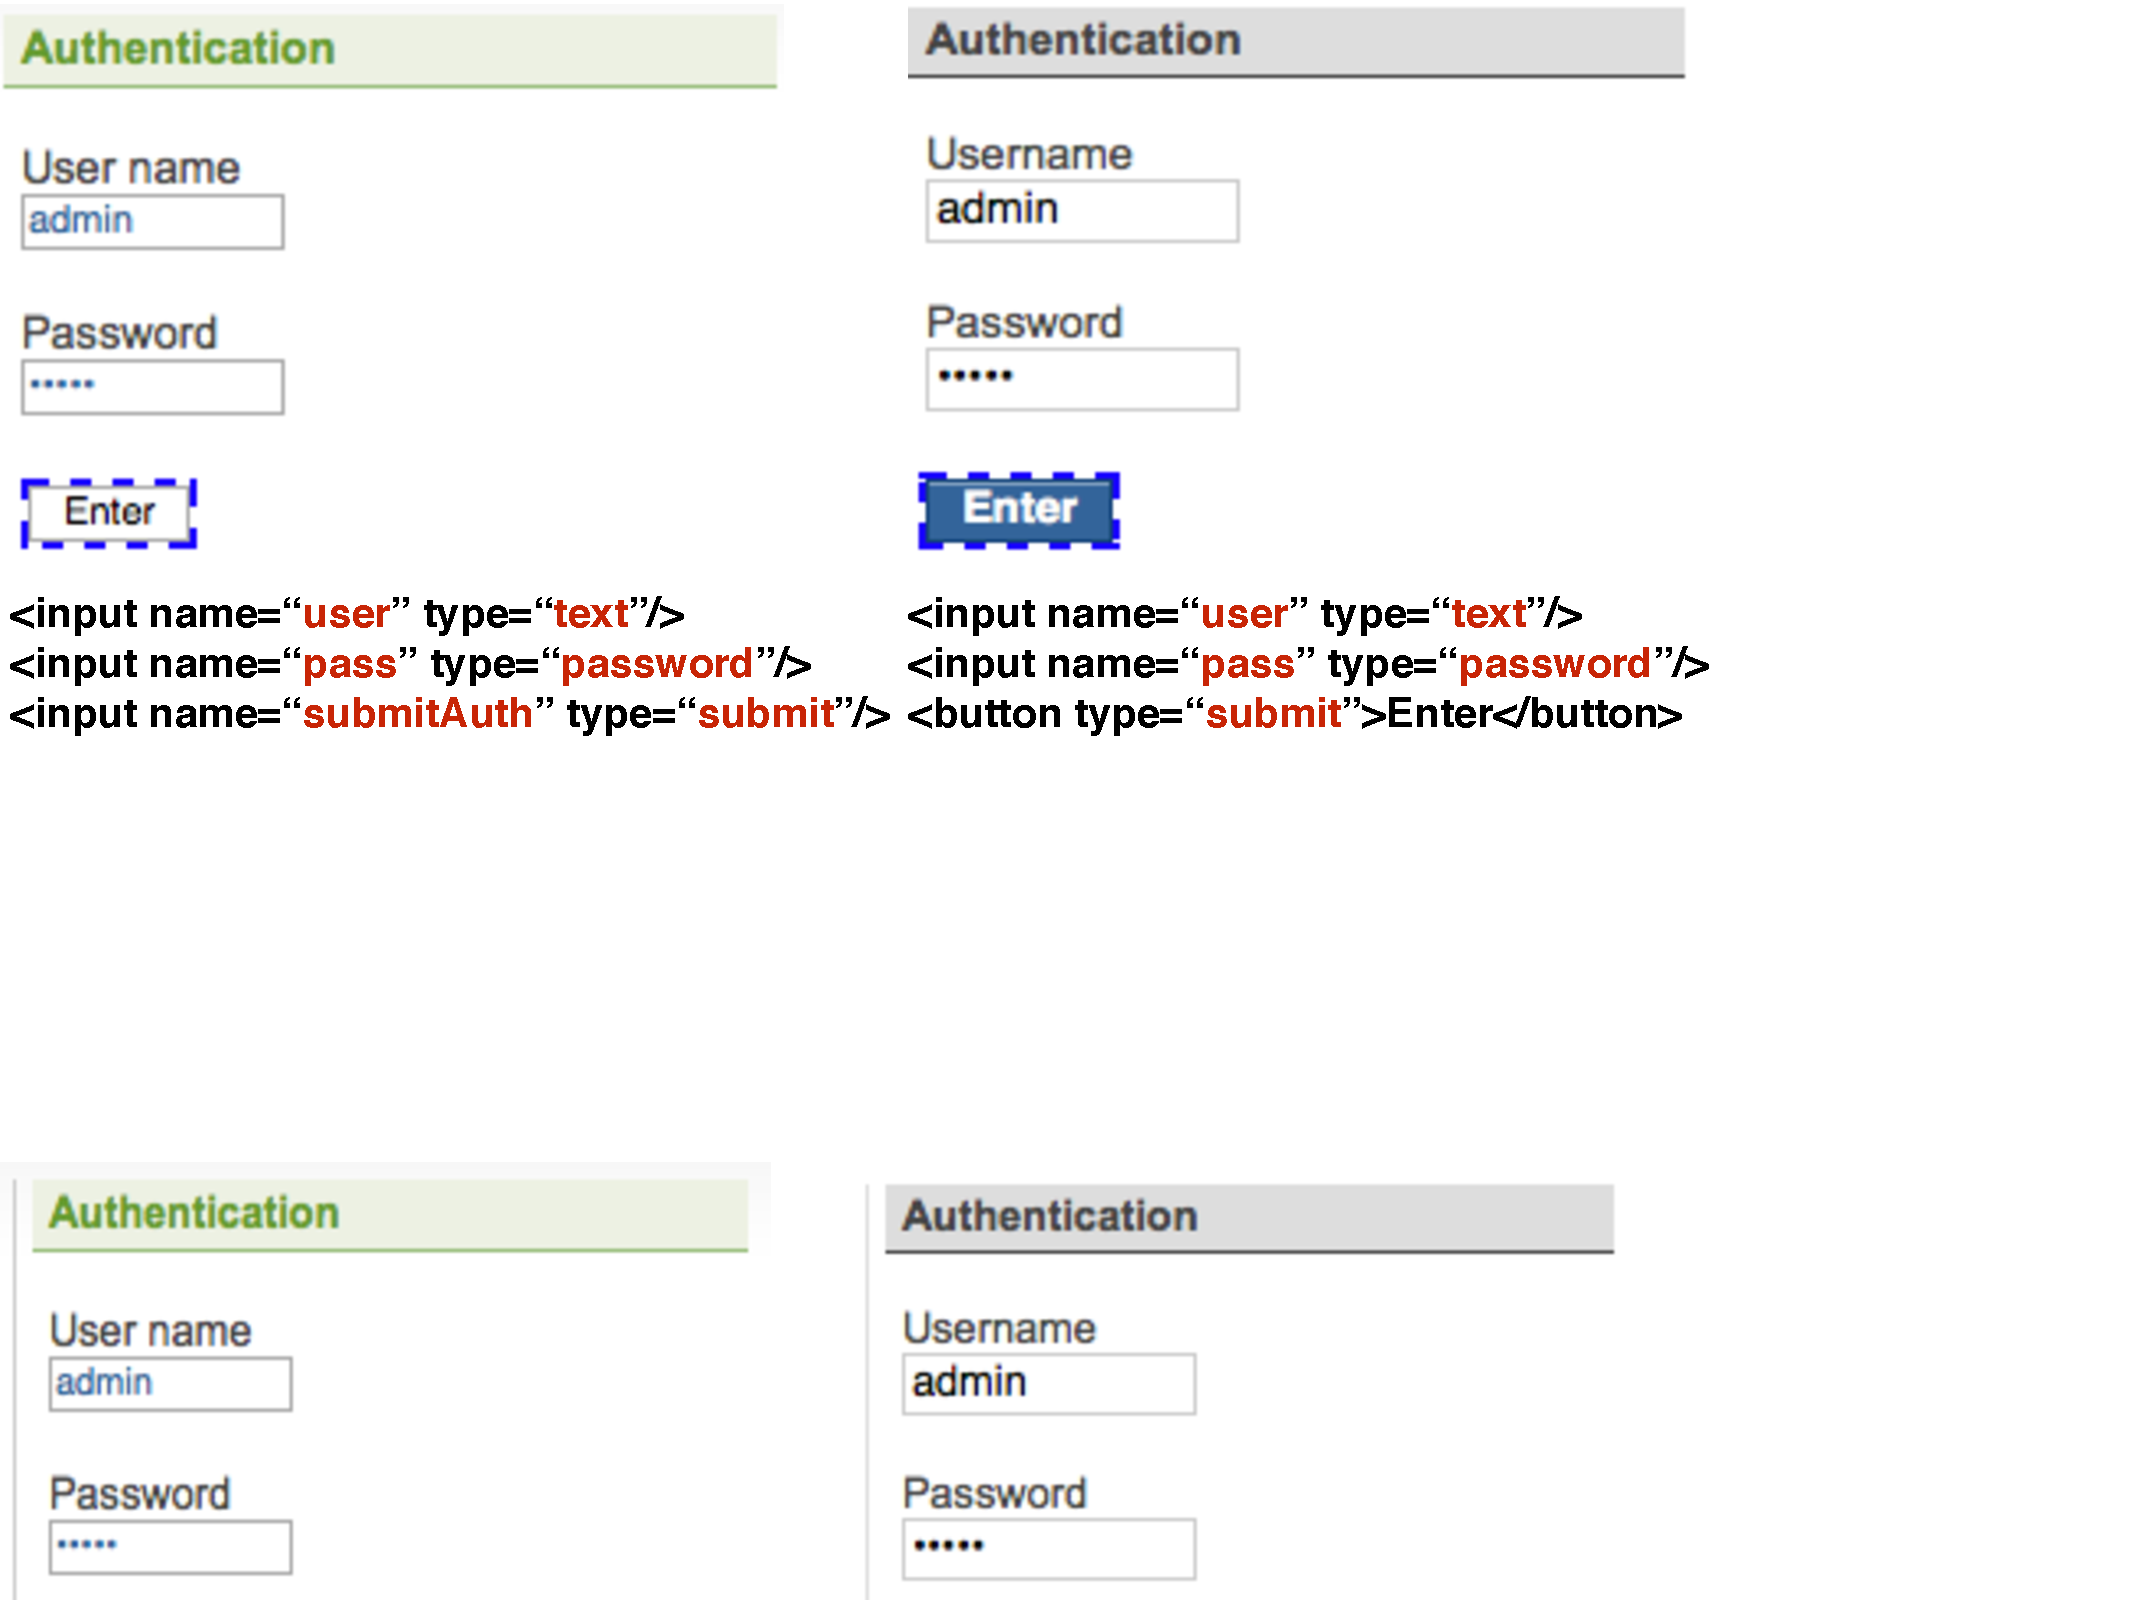
\includegraphics[trim={0cm 14cm 7.1cm 0cm},clip,scale=0.29]{images/claroline2}
%%}
%\caption{Login page of the Claroline web application, version 1.10.0 (left) and version 1.11.0 (right), along with a portion of the corresponding HTML code}
%\label{claroline}
%\end{figure}

%\begin{figure}[t]
%\centering
%%\fbox{
%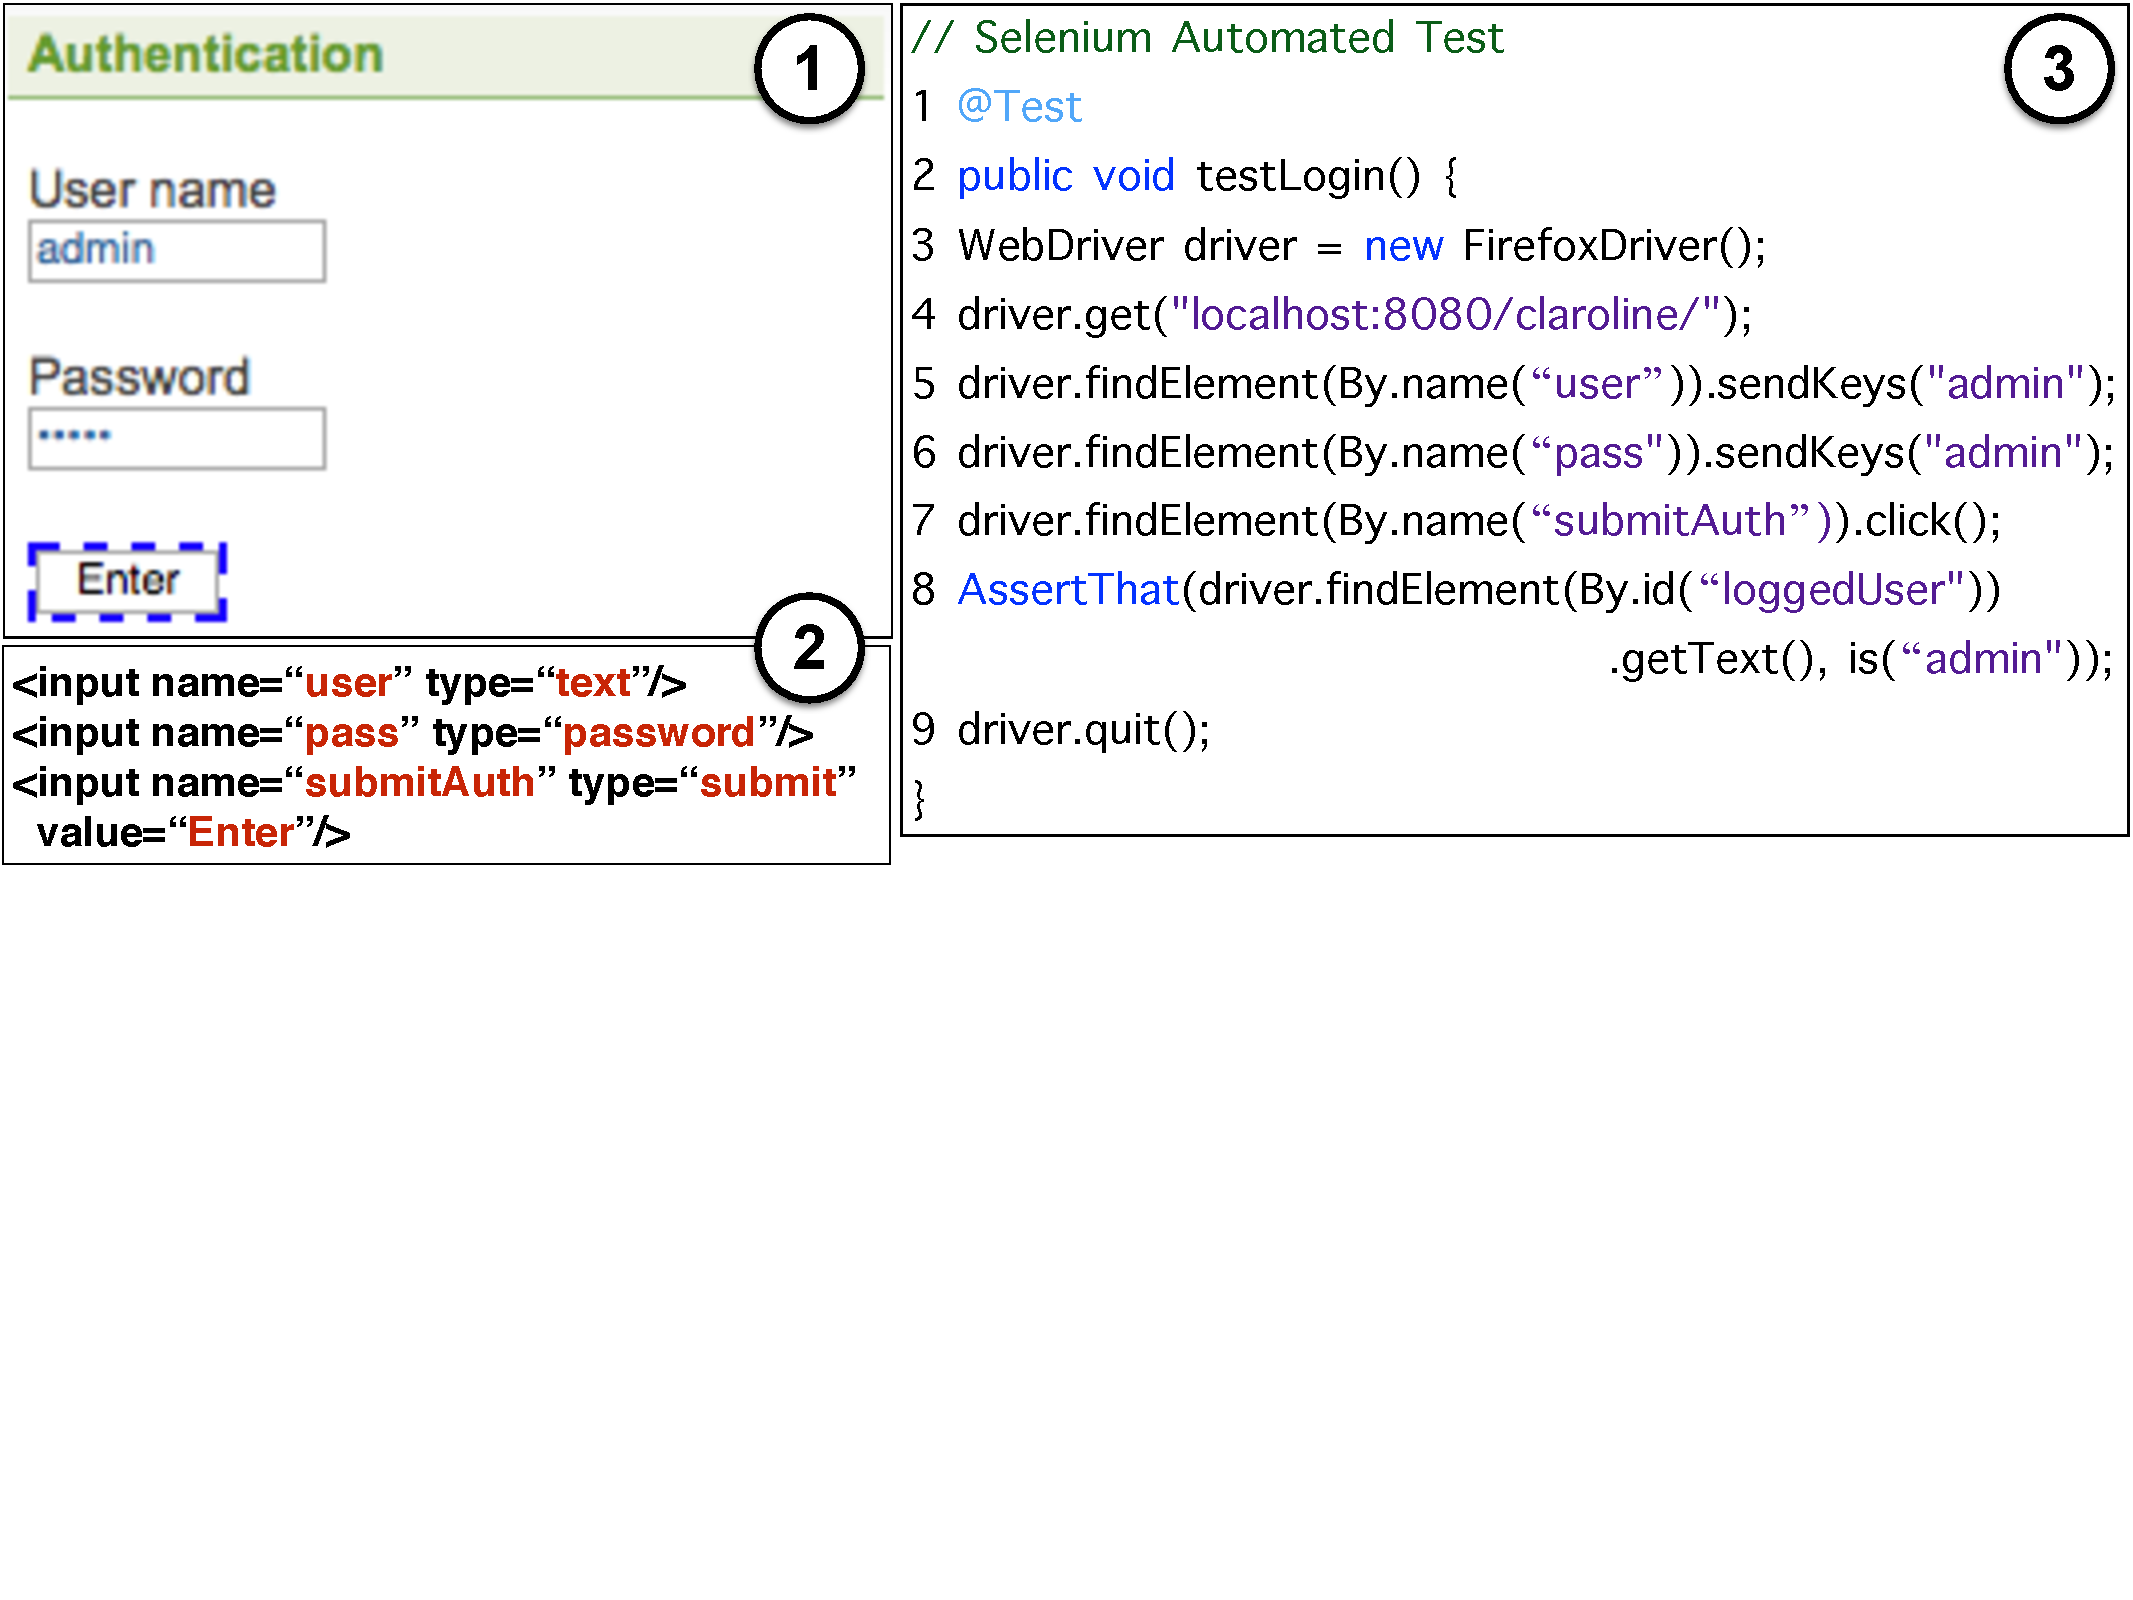
\includegraphics[trim={0cm 12.4cm 0cm 0cm},clip,scale=0.23]{images/claroline-version1}
%%}
%\caption{Login page of the Claroline web application (version 1.10.0), along with a portion of the corresponding HTML code, and an automated Selenium test}
%\label{claroline-version1}
%\end{figure}

%In presenting the basic knowledge to understand the remainder of the paper, we use as running example the real world web application Claroline~\cite{claroline}, one of the experimental objects used in our study. 
%\autoref{claroline-version1}~\textcircled{\raisebox{-0.9pt}{1}} shows the login form of Claroline version 1.10.0, together with the corresponding HTML code~\textcircled{\raisebox{-0.9pt}{2}}.
%
%Let us a test scenario in which a user 
%inserts \texttt{username} and \texttt{password} 
%in the login form, and if these credentials are correct, 
%the \texttt{username} is displayed on the the homepage (not shown for brevity).
%%
%\autoref{claroline-version1}~\textcircled{\raisebox{-0.9pt}{3}} shows an automated test case implementing such scenario, developed using the popular Selenium framework~\cite{}.
%In Line~3, an instance of WebDriver is 
%created to control the Firefox browser. 
%In Line~4, the executable test case instruments WebDriver to 
%navigate to the URL of the target web application.  
%Lines~5-6 fill in the username and password input boxes 
%with the administrator credentials, and Line~7 submits the form. 
%Line~8 verifies, by means of an assertion, the presence 
%of an HTML element containing the username in the home page, 
%and asserts that it equals the string ``admin''. 
%Finally, Line~9 shuts down the WebDriver instance 
%and closes the browser.

In this section, we present basic concepts
about E2E test automation that are needed 
to understand the remainder of the paper.
We provide background information on 
DOM-based and visual web testing approaches.
To help present these approaches and concepts
we use the example provided in~\autoref{fig:ab-back}: 
a simplified version of the AddressBook web application, 
one of the experiment objects used in our study. 
We consider a scenario in which a user 
inserts a \texttt{username} and \texttt{password} 
in the AddressBook login form 
(\autoref{fig:ab-back-a}), 
and if these credentials are correct, 
the \texttt{username} (\texttt{`admin'}) is displayed on the top right corner of the homepage 
(\autoref{fig:ab-back-b}).

\subsection{Approaches to E2E Test Automation}
In recent years, two major approaches to E2E web testing have emerged, each of them associated with a diverse way of interacting with the AUT. 

\begin{table}[b]
\setlength{\tabcolsep}{3pt}
\renewcommand{\arraystretch}{1}
\centering
\caption{An example of C\&R automated test (Selenium IDE)}
\begin{tabular}{cclc}
\toprule
\textbf{Line} & \textbf{Action}   & \textbf{Locator} & \textbf{Value} \\
\midrule
1 & open             & localhost/addressbook/index.php &                \\
2 & type             & name=user                         &  ``admin''   \\
3 & type             & name=pass                         &  ``secret'' \\
4 & click            & id="submitLogin"                           &           \\
5 & assertText  & id="loggedUser"                           &   ``(admin)''        \\
\bottomrule
\end{tabular}
\label{t:seleniumtest}
\end{table}

\textbf{DOM-based} tools access and inspect properties of the Document Object Model (DOM), the hierarchical structure underlying a web page. To this category belong capture-replay (C\&R) and programmable tools. \textit{Capture-replay} tools are based on the recording of sequences of inputs and actions performed by the tester on the web application GUI. The recording process creates a test script (see~\autoref{t:seleniumtest}) that can be replayed in a unattended mode. 
With \textit{programmable} tools, on the other hand, test cases themselves become software artefacts that developers write 
resorting to specific testing frameworks (see~\autoref{lst:login-no-abs-back}). The framework API supports the automated interaction with a web page and its elements, so that test cases can, for instance, automatically fill-in and submit forms or click on hyperlinks. There are many C\&R tools for web applications available, e.g., Selenium IDE~\cite{selenium}, Sahi~\cite{sahi}, and Ringer~\cite{ringer}. A representative of the programmable category is Selenium WebDriver~\cite{selenium}, which is considered the flagship open-source test automation tool for web applications.

\begin{lstlisting}[firstnumber=1, xrightmargin=6ex, float=t,numbers=right,caption={An example of programmable automated test (Selenium WebDriver)},label=lst:login-no-abs-back]
@Test
public void testLogin(){
	WebDriver driver = new FirefoxDriver();
	driver.get("localhost/addressbook/index.php");
	driver.findElement(By.name("user")).sendKeys("admin");
	driver.findElement(By.name("pass")).sendKeys("secret");
	driver.findElement(By.id("submitLogin")).click();
	AssertThat(driver.findElement(By.id("loggedUser")).getText(), contains("admin"));
	driver.quit();
}
\end{lstlisting}

An emerging and relatively new approach is \textbf{visual} web testing, in which the AUT is tested through its GUI. Indeed, the emergence of new complex visual components in web pages has required new ways of interfacing with the web applications. Visual tools such as JAutomate~\cite{Alegroth2013jat}, Sikuli~\cite{Sikuli}, and EggPlant Functional~\cite{eggplant} use image recognition techniques to identify the web elements displayed on the web page (see~\autoref{fig:visual}). Visual web testing tools offer an interesting alternative, promising easier and more intuitive test case creation, and they are increasingly being adopted also in industry~\cite{Alegroth2013jat}. 
%and in general, they can be considered as a valid choice in all cases where testers have to deal with highly visual interactive applications, such as Google Maps. 
\autoref{fig:visual} shows the visual version of the DOM-based test of~\autoref{lst:login-no-abs-back}, developed using Sikuli~\cite{Sikuli}. We can notice how web elements are localised by \textit{visual locators}, i.e., images representing a portion of the GUI. Thus, elements are characterised by their visual appearance, instead of a DOM-based locator.

\begin{figure}[b]
\centering
\fbox{
{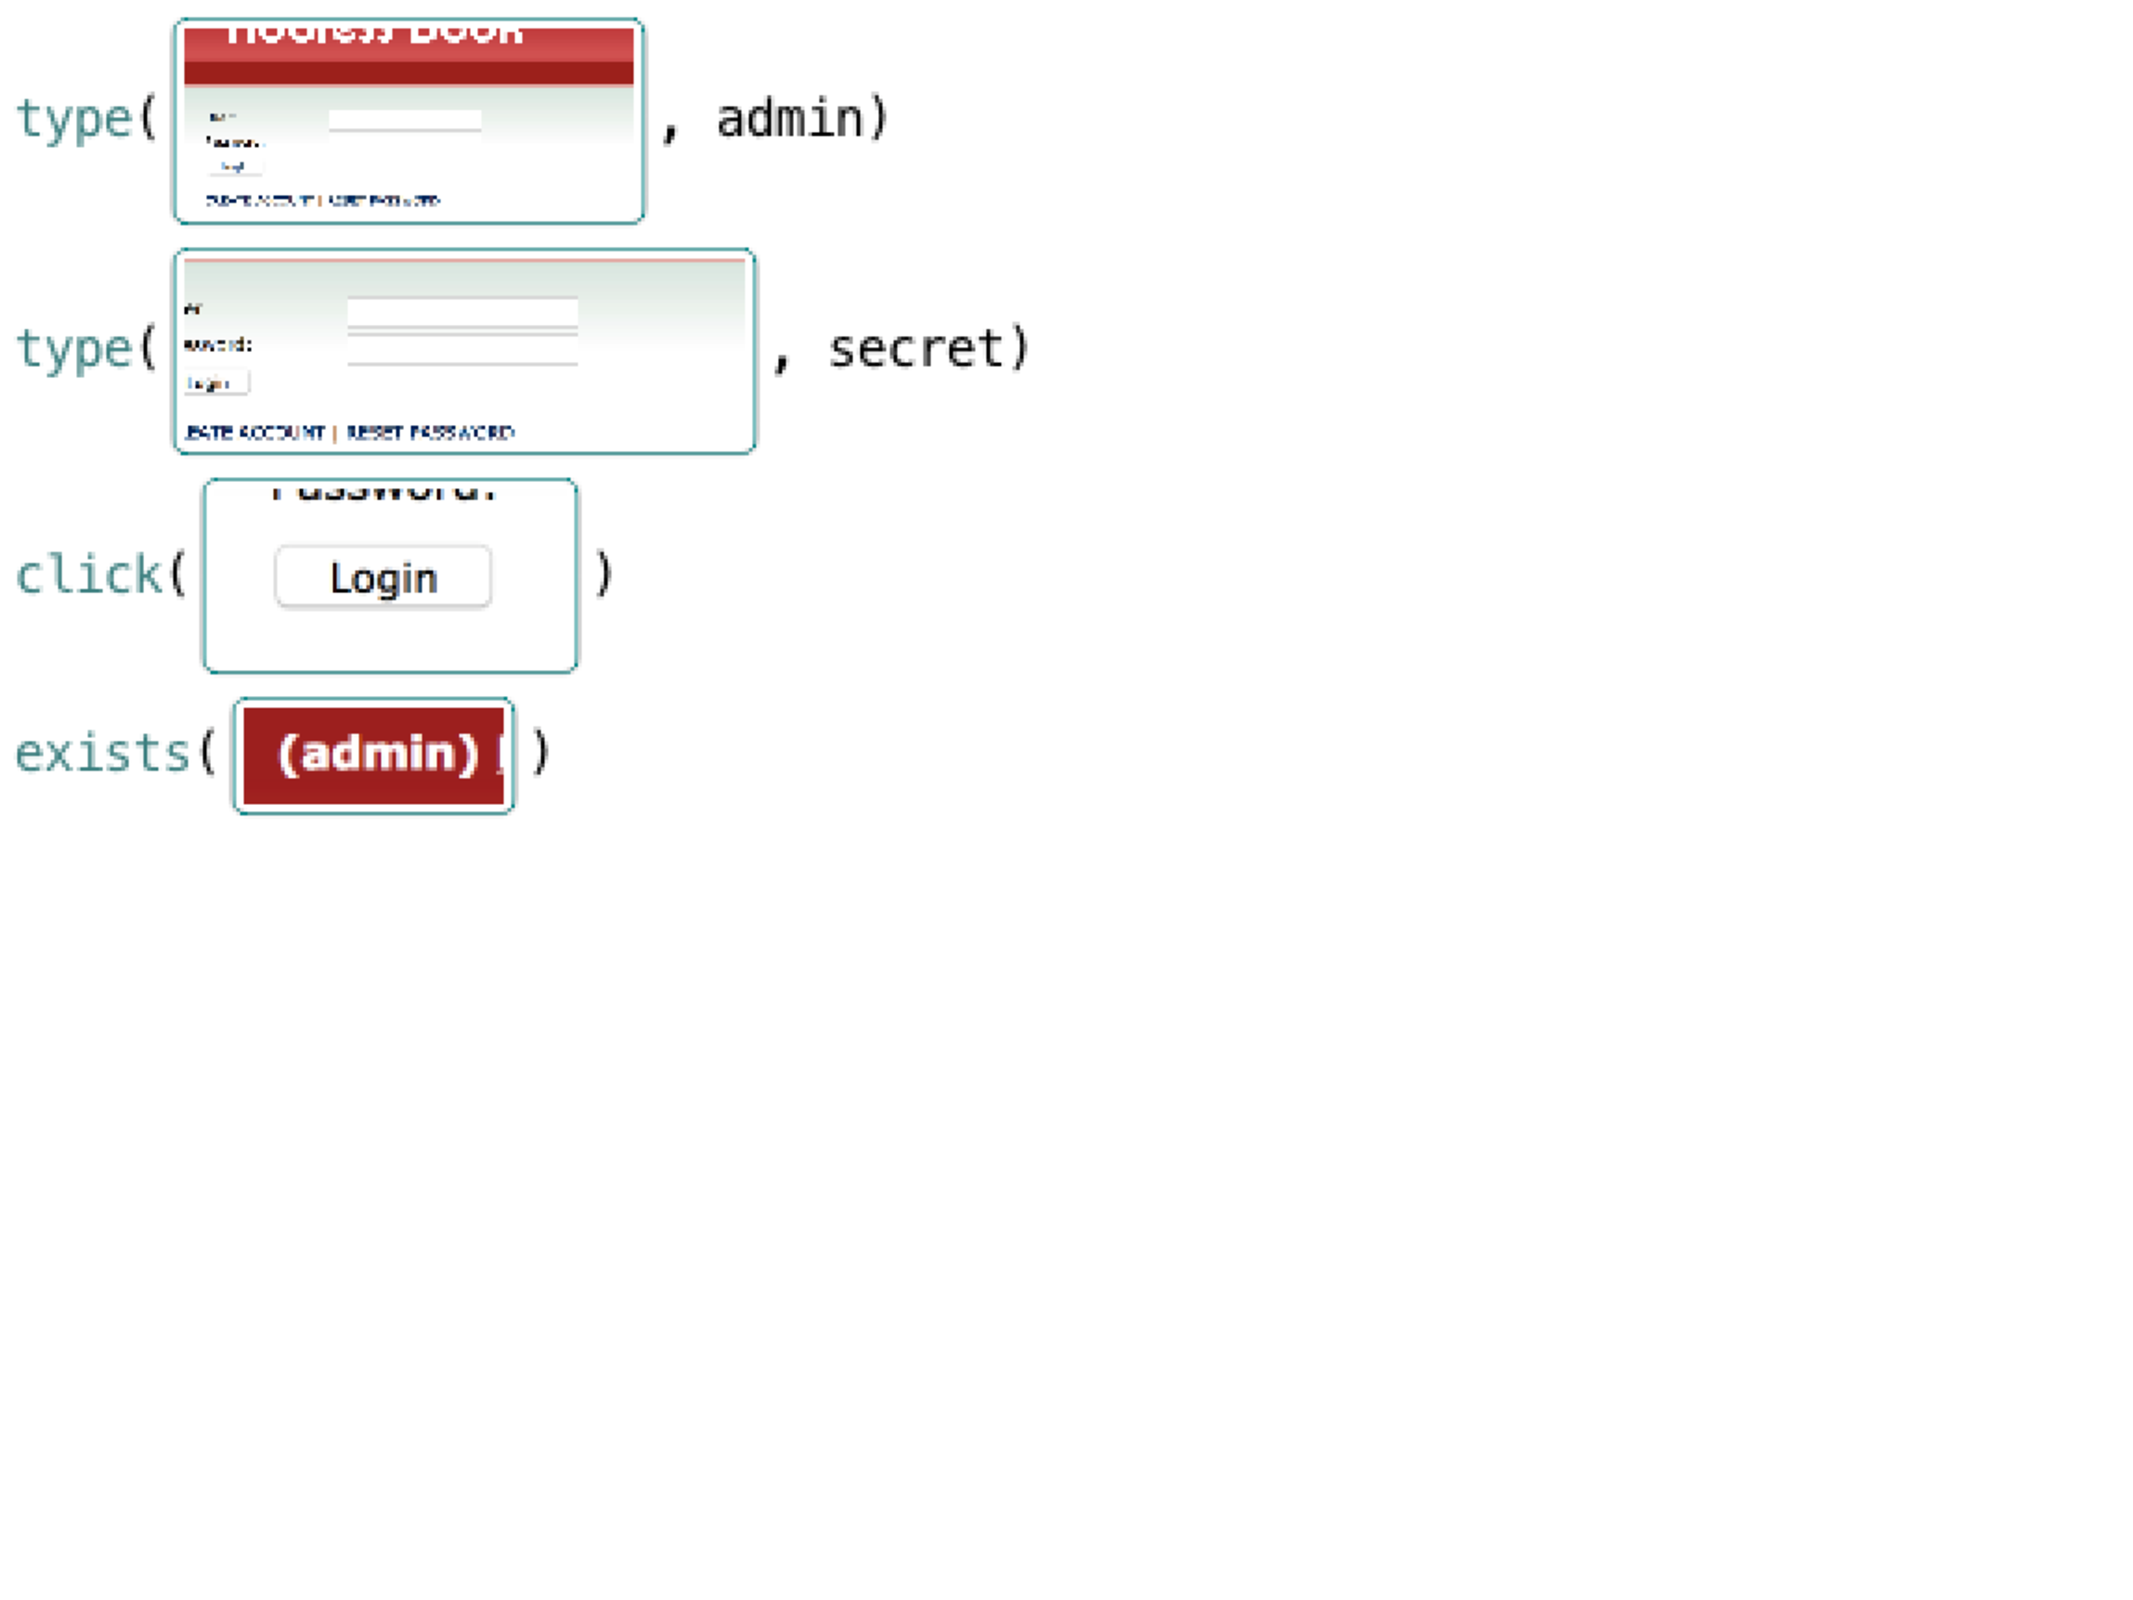
\includegraphics[trim=0.1cm 13cm 19cm 0.1cm, clip=true, scale=0.28]{images/sikuli-s.pdf}}
}
\caption{An example of visual automated test (Sikuli)}
\label{fig:visual}
\end{figure}

\subsection{The Dilemma}
Both approaches come with advantages and disadvantages, and are quite utilized. %, given the plethora of existing solutions for both categories. Among the DOM-based tools we recall \ldots~\cite{}, whereas for the visual approach we recall \ldots~\cite{}.
To date, however, both approaches coexist and it is not clear whether one will eventually prevail over the other. Our intuition behind this uncertain scenario is that, depending on the kind of AUT, both the DOM-based and the visual approaches to web testing have their own advantages. For instance, for highly interactive web applications such as Google Maps, the DOM can be complicated to retrieve, thus it is more convenient to rely on a visual testing tool that is capable of asserting on the correctness of the web page visual content.
In addition, DOM-based tools do not take into account the visual appearance of the AUT, which is instead important because it is used by the tester as the main oracle against which to evaluate the correctness of the software. Visual tools, on the other hand, completely abstract away the model of the page, and create actions and assertions in a purely visual manner. 
%
Hybrid approaches such as Applitools~\cite{applitools} try to unify the two approaches and allow a tester to manually inject visual checks at specific points of the test execution. This has two drawbacks: (1)~the insertion of the check-points must be performed manually, (2)~this extra-code clutters the initial test code, with statements that do not pertain to the test scenario itself.

\head{The Idea}
We believe that the use of visual technologies would be especially beneficial for regression testing purposes, rather than for test creation. For example, the GUI can be used to verify the correct execution of the tests as the AUT evolves over time (in a similar way as testers do), or to detect deviations from the correct behaviour.
Indeed, E2E tests are mostly used in \textit{regression} scenarios, i.e., to verify that the most recent code changes have not adversely affected existing features. To do so, already existing test cases are re-executed to ensure that the current functionalities still work correctly. 
%
Unfortunately, web tests are well-known to be very fragile in the face of software evolution~\cite{2016-leotta-Advances,2016-Leotta-JSEP,Hammoudi-2016-ICST}. %Indeed, automated test code is usually highly coupled with low-level implementation details such as HTML attributes and thus result fragile and difficult to maintain as the AUT evolves~\cite{2016-leotta-Advances,2016-Leotta-JSEP,Hammoudi-2016-ICST}. 
Even a minor GUI change might break a previously developed test case, whose script would need to be repaired manually, or re-written to match the new version of the web application, even if conceptually the functionality is unaltered, and no errors are present in the production code.

\subsection{Existing Web Tests Repair Approaches}

Test repair techniques have been proposed in the last years~\cite{Gao:2016:SGT:3046547.3046580,Daniel:2011:AGR:2002931.2002937,Daniel:2009:RSR:1747491.1747538,Daniel:2010:TRU:1831708.1831734,Choudhary:2011:WWA:2002931.2002935,Hammoudi-2016-FSE}. However, only a few proposals target the web domain. To date, the state of the art web test repair algorithm is \water, by Choudhary et al.~\cite{Choudhary:2011:WWA:2002931.2002935}. \water is based on differential testing, and compares the correct test execution with the failing one in order to find potential fixes for the broken tests. While the repair algorithm of \water has a straightforward design and can manage a good number of cases related to locators or assertions, it has a number of limitations that derive from its  DOM-related narrowness: First, this can lead to a great number of false positives, as recognized by the authors of the paper~\cite{Choudhary:2011:WWA:2002931.2002935}. Second, 
 relying only on the DOM may be insufficient to find candidate repairs. Third, the algorithm does not reflect the way in which testers attempt at repair tests, an activity that often requires to inspect the GUI of the two applications in order to find the root causes of the breakages. Fourth, it relies on the assumption that the repair has always to be triggered at the point in which the test stops, which makes it impossible to handle propagated breakages~\cite{Hammoudi-2016-ICST}, i.e., cases in which a breakage appears in a later point of the test execution. In many of such cases, it is imperative for the tester to inspect the GUI.

%\subsection{Definitions} At a high level, each Selenium command is a tuple \textit{<locator, action, value>}. A locator is a function on a DOM state $D$, as follows, $$l: D \rightarrow e$$ where $e$ is the target element returned by the locator $l$ when applied to $D$. \andrea{to decide if and what to include}

%\begin{figure*}[t]
%\centering
%\includestandalone[width=\textwidth]{forest}
%\caption{Taxonomy of locator-based test case breakage scenarios in the web domain}
%\label{fig:taxonomy}
%\end{figure*}
%\begin{figure}[b]
%\centering
%\includestandalone[width=\columnwidth]{forest}
%\caption{Taxonomy of locator-based test case breakage scenarios in the web domain}
%\label{fig:taxonomy}
%\end{figure}


%\subsection{Testers Mental Model when Repairing Web Tests}
%
%When a breakage occurs, a tester tries to understand the root cause behind the breakage and a possible repair by inspecting and linking the behaviour of three entities, namely 1) the test code, 2) the GUI, 3), the DOM. 
%Moreover, web test cases such as Selenium's are arguably more difficult to repair than standard JUnit tests for desktop applications, because
%Selenium's APIs and JUnit error stack trace messages are usually poorly informative for the tester or can be totally deceiving for detection purposes.
%
%In doing so, this activity involves at least four steps: 
%(1)~the tester inspects the error stack trace or the console, which may contain information about the origin of breakage (e.g., ``\texttt{NoSuchElementException} occurred. Unable to locate element with XPath \mbox{\texttt{html/body/div[1]/label}}''). 
%(2)~the tester inspects $t$ to find the statement $st$ responsible for the failure; %which is also likely to be the one that needs to be corrected (note that this is not always true).
%(3)~the tester navigates the GUI of $V'$, trying to identify the portion of the GUI which is related to $st$. 
%(4)~depending on the kind of breakage, the tester inspects either the (i)~DOM of $V'$, or (ii)~the GUI of $V'$, or (iii)~both the DOM and the GUI, to find candidate repair solutions. In doing so, the tester may possibly need to exercise manually the same broken scenario of $t$, in order to replicate the breakage occurred at $st$ and gather insights on possible repair actions.
%
%Thus, in other words, breakages are often repaired by finding candidate solutions by inspecting the DOM and the GUI \textit{at the same time}. However, this task can be boring, time-consuming, and among all challenging. Existing test automation tools offer no support in understanding the root causes behind test breakages and how they do relate with the changes made in the web applications. In this paper we wish to make step ahead to provide such understanding. 
%Our aim is to combine the knowledge present in the DOM of the application with its visual appearance, so as to effectively aid the tester in the test repair problem. Our approach aims at automating  the mental model the testers create when a test case is executed against a web application GUI. In our belief, such a model is a viable means for automatic test case repair.

%Table~\ref{table:rootcauses} presents different breakage scenarios, in which we correlate all the findings from the aforementioned previous research, with the purpose of gaining more understanding of the type of breakages and the effects they have on the web application and the related test repairs. Column 1 of the table lists the distal causes (i.e., modification to the web app under test), column 2 describes the proximal causes~\cite{Hammoudi-2016-ICST} (i.e., the portion of the test impacted by the distal cause), and the last macro-column (Impact) illustrates whether the breakage impacts the web app DOM, its GUI or the test workflow, respectively. In the table, breakages causes have been further categorized in three meta-categories: Addition, Deletion, and Modification, depending on the kind of evolution underwent on the web application.

%\subsection{Test Breakage Scenarios}
%
%In doing so, he typically performs three tasks. First, 
%
%
%When a breakage occurs, Selenium's APIs and JUnit error stack trace messages are usually poorly informative for the tester or can be totally deceiving for detection purposes. Here we present recurring breakage scenarios that are that either 1) challenging to detect, or 2) impossible to repair with existing automatic techniques. We will also show how the visual inspection can help to mitigate such problems.
%
%\textit{Scenario 1 --- Web Application Evolution}. 
%Let us consider \autoref{claroline-version1} again. 
%When executed on version 1.11.0~(right), the test will stop at Line~7 when attempting to locate the ``Enter'' button (highlighted in blue in the figure), because the attribute \mbox{\texttt{name="submitAuth"}} has been removed from the page. One may attempt to use another locator, such as the XPath of the element. Unfortunately, due to a drastic change in the structure underneath the web page, even the tag of the element has changed (from \mbox{\texttt{input}} to \mbox{\texttt{button}}).
%However, it is evident that \textit{visually} the target element is still present, and its position on the GUI has not changed. 
%At a visual inspection of the two GUIs, a tester would expect this test to work, because his/her perception is immaterial where changes at DOM-level are concerned.

%%\begin{figure}[t]
%%\centering
%%%\fbox{
%%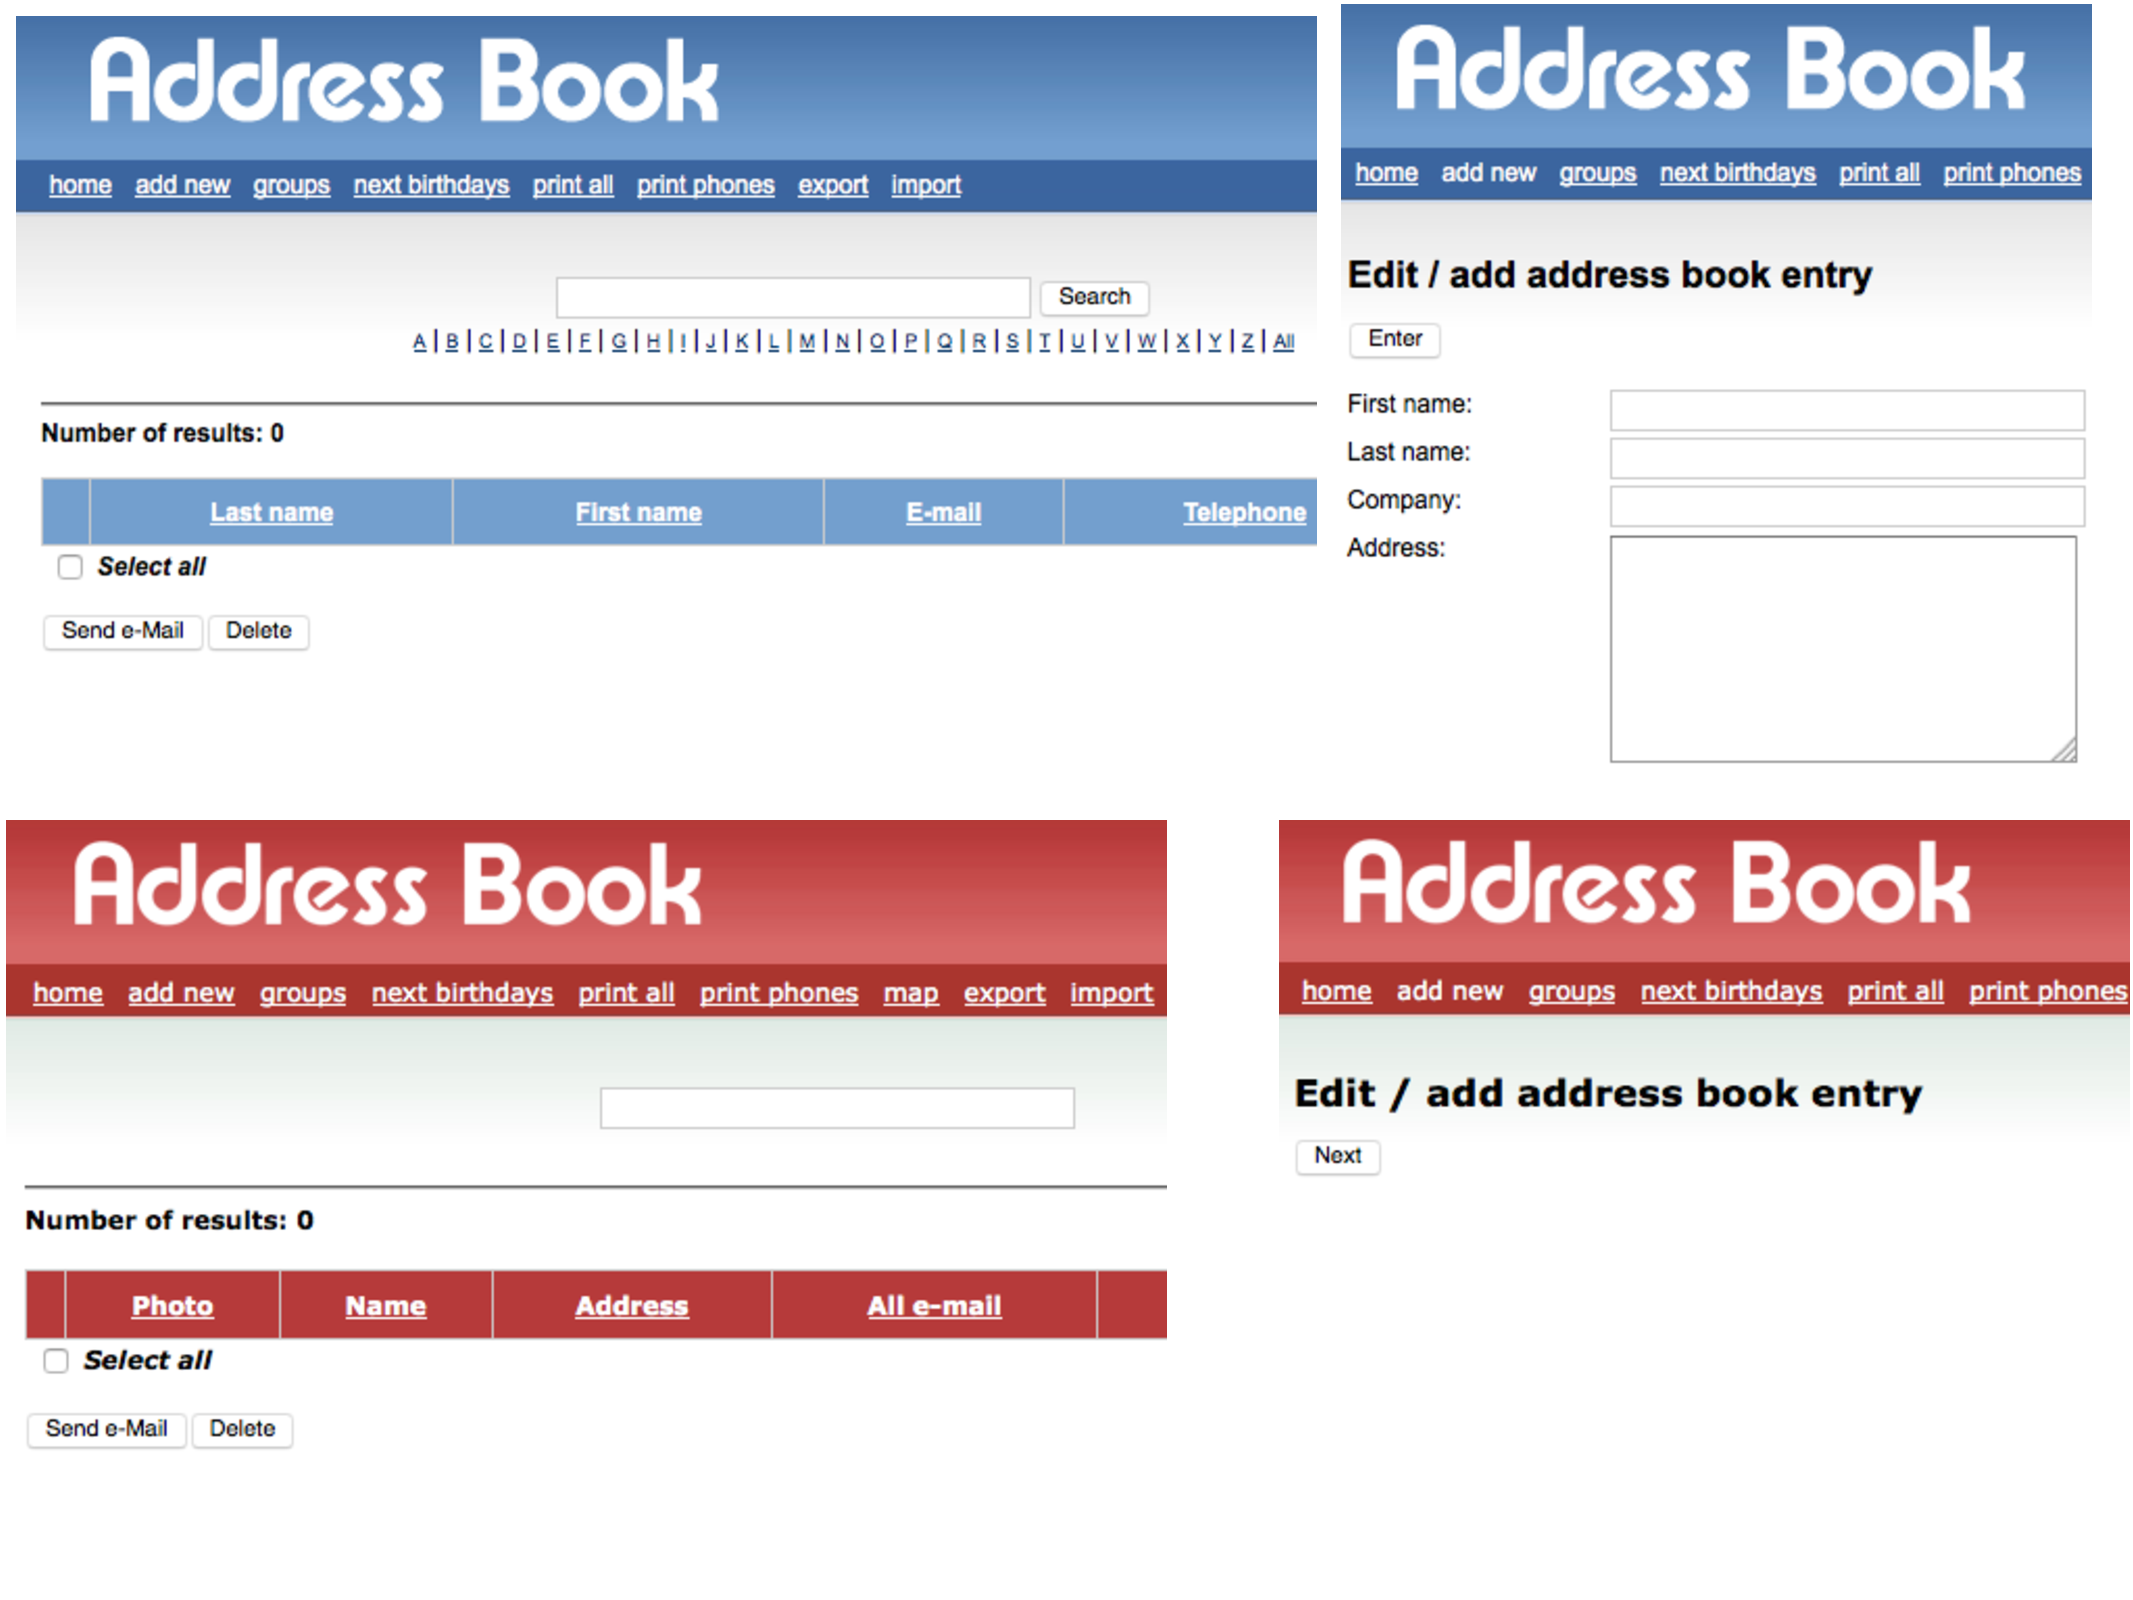
\includegraphics[trim={0cm 2cm 0cm 0cm},clip,scale=0.2]{images/addressbook}
%%%}
%%\caption{AddressBook}
%%\label{addressbook}
%%\end{figure}
%
%\textit{Scenario 2 --- Mis-Selection or Propagated Breakage}.
%We focus on solving the problem due to propagated breakages  because it is very common in web testing due to locators mis-selection. 
%
%We want to make sure that all the locators select the correct elements, respectively.
%
%Two variants: the mis-selection does not cause a state transition (the app remains in the same state), or it does trigger a state transition and leads to a different state.




